\documentclass[11pt]{article}
\usepackage[T1]{fontenc}
\usepackage[utf8]{inputenc}
\usepackage{lmodern}
\usepackage[margin=1in]{geometry}
\usepackage{amsmath,amssymb,amsthm}
\usepackage{booktabs,array,graphicx}
\usepackage{microtype,parskip}
\usepackage[numbers,sort&compress]{natbib}
\usepackage{xcolor}
\usepackage{url}
\usepackage[colorlinks=true,linkcolor=teal,citecolor=teal,urlcolor=teal]{hyperref}
\usepackage{fancyhdr}
\usepackage{placeins}
\definecolor{teal}{RGB}{0,108,115}
\hypersetup{pdftitle={Hypercomplex Coordinates and Finite Feedback Dynamics in SHA-3 Cryptanalysis},
pdfauthor={Kaoru Aguilera Katayama},pdfsubject={Reproducible reduced-round SHA-3 cryptanalysis},
pdfkeywords={SHA-3, Keccak, Clifford algebra, Markov models, Tarjan, 2-SAT}}
\pagestyle{fancy}
\fancyhf{}
\fancyhead[L]{\small Hypercomplex and finite-feedback SHA-3 analysis}
\fancyhead[R]{\small K. Aguilera Katayama}
\fancyfoot[C]{\thepage}
\setlength{\headheight}{14pt}
\setlength{\emergencystretch}{2em}
\newtheorem{proposition}{Proposition}
\newtheorem{definition}{Definition}
\newcommand{\Cl}{\operatorname{Cl}}
\newcommand{\HW}{\operatorname{HW}}
\newcommand{\Maj}{\operatorname{Maj}}
\newcommand{\E}{\mathbb{E}}
\newcommand{\F}{\mathbb{F}}
% Generated by scripts/build_report.py; do not edit numbers.
\newcommand{\CollisionDigest}{0c000000003400000000000000000000\\
00000000003400000d00000000000000}

\newcommand{\DiffusionTable}{%
\begin{tabular}{rrrrr}
\toprule
Rounds & State $K$ & State $C$ & Digest $K$ & Digest $C$ \\
\midrule
1 & 4.009 & 40.023 & 0.000 & 7.508 \\
2 & 82.113 & 525.995 & 13.034 & 78.920 \\
3 & 692.113 & 800.554 & 109.723 & 128.045 \\
4 & 799.902 & 799.693 & 128.020 & 127.932 \\
6 & 800.371 & 799.953 & 128.079 & 128.112 \\
12 & 799.647 & 799.705 & 127.942 & 127.999 \\
24 & 800.098 & 800.060 & 127.989 & 127.992 \\
\bottomrule
\end{tabular}%
}

\newcommand{\AUCTable}{%
\begin{tabular}{rrrr}
\toprule
Rounds & Hamming & Clifford grades & Combined \\
\midrule
1 & 1.0000 & 1.0000 & 1.0000 \\
2 & 1.0000 & 1.0000 & 1.0000 \\
3 & 0.9901 & 0.5661 & 0.9885 \\
4 & 0.4892 & 0.4879 & 0.4884 \\
6 & 0.4835 & 0.4831 & 0.4811 \\
12 & 0.4896 & 0.4919 & 0.4906 \\
24 & 0.5129 & 0.4877 & 0.4897 \\
\bottomrule
\end{tabular}%
}

\newcommand{\MarkovTable}{%
\begin{tabular}{lrr}
\toprule
Predictor & Bits / transition & 95\% interval \\
\midrule
Phase only & 1.097400 & [1.092665, 1.102134] \\
First-order bins & 1.092961 & [1.088188, 1.097734] \\
Dyadic, no feedback & 1.076552 & [1.071993, 1.081110] \\
Dyadic, self-feedback & 1.079077 & [1.074225, 1.083929] \\
\bottomrule
\end{tabular}%
}

\newcommand{\CausalTable}{%
\begin{tabular}{rrrr}
\toprule
Rounds & Mean $I_{ij}$ & Mean $|A_{ij}|$ & Mean $|\rho_{ij}|$ \\
\midrule
1 & 0.5994 & 0.0095 & 0.0121 \\
2 & 0.5002 & 0.0090 & 0.0128 \\
3 & 0.5001 & 0.0083 & 0.0125 \\
4 & 0.5002 & 0.0088 & 0.0124 \\
6 & 0.5003 & 0.0085 & 0.0119 \\
12 & 0.5005 & 0.0092 & 0.0130 \\
\bottomrule
\end{tabular}%
}

\newcommand{\CyclesTable}{%
\begin{tabular}{rrrr}
\toprule
Rounds & Cycles & Cyclic vertices & Longest cycle \\
\midrule
1 & 5 & 140 & 79 \\
2 & 5 & 113 & 78 \\
12 & 1 & 25 & 25 \\
\bottomrule
\end{tabular}%
}

\newcommand{\SearchTable}{%
\begin{tabular}{rrrrr}
\toprule
Rounds & Random & Full model & Exact $p$ & Holm $p$ \\
\midrule
2 & 21/48 & 38/48 & 0.00151 & 0.00454 \\
3 & 24/48 & 15/48 & 0.07835 & 0.15671 \\
24 & 16/48 & 24/48 & 0.15159 & 0.15671 \\
\bottomrule
\end{tabular}%
}

\newcommand{\AblationTable}{%
\begin{tabular}{lrrrr}
\toprule
Method & $r=2$ hits & Queries & $r=24$ hits & Queries \\
\midrule
Random & 22/48 & 1546.4 & 21/48 & 1576.6 \\
Hill climbing & 25/48 & 1435.7 & 17/48 & 1641.8 \\
No self-feedback & 35/48 & 1141.2 & 19/48 & 1669.8 \\
Stagnation restart & 33/48 & 1098.8 & 21/48 & 1575.6 \\
Full model & 34/48 & 1111.5 & 21/48 & 1591.2 \\
\bottomrule
\end{tabular}%
}


\title{\textbf{Hypercomplex Coordinates and Finite Feedback Dynamics in SHA-3 Cryptanalysis}\\[0.45em]
\large Exact representations, reduced-round attacks, and Tarjan graph analysis}
\author{Kaoru Aguilera Katayama}
\date{October 11, 2026 (UTC)\\
\small Code and data: \url{https://github.com/PolloXDDD/SHA3-ANALISIS}}

\begin{document}
\maketitle
\begin{abstract}
We investigate three proposed routes to SHA-3 cryptanalysis: hypercomplex state representations, finite self-referential Markov models with dyadic structure, and cycle analysis using Tarjan's algorithm together with Boolean interventions and displacement metrics. Each 64-bit lane is embedded exactly in the real Clifford algebra $\Cl(0,6)$. We derive the transported Boolean operations and prove that the resulting coefficient distance contains exactly the information of Hamming distance. A column-parity construction gives a universal collision family for a one-prefix-round SHA3-256 variant, with an explicit certificate. Experiments on 8,192 message pairs per difference show strong early-round diffusion structure, followed by near-half-state displacement. Held-out Clifford features, finite-feedback prediction, exhaustive projected cycles, and an exact local 2-SAT obstruction are evaluated separately. A combined search finds 38 of 48 twelve-bit targets at two rounds, compared with 21 for random search under the same query cap; an independent replication finds 34 versus 22. Ablations do not establish a separate benefit from self-reference or SCC checks. At 24 rounds the replication gives 21 successes for both methods. These results identify tractable reduced-round structure and precisely delimit what the proposed representations and graph reductions preserve. No full-output, full-round collision or preimage attack is obtained.
\end{abstract}

\noindent\textbf{Keywords:} SHA-3; Keccak; Clifford algebra; finite Markov model; differential cryptanalysis; strongly connected components; Boolean influence.

\section{Question, scope, and prior work}

The question is whether alternative coordinates and finite feedback can expose useful structure in SHA-3's nonlinear dynamics. We operationalize three research directions: (i) genuinely hypercomplex algebra, (ii) self-referential transition models with a repeated finite-scale rule, and (iii) graph cycles, 2-SAT implications, interventions, and displacement. The aim is to obtain verifiable mathematical statements and attack measurements from these ideas.

The target is the byte-aligned SHA3-256 construction in FIPS~202~\cite{fips202}. Its permutation has 1,600 bits arranged in 25 lanes of 64 bits. Our software also implements the other three SHA-3 digest lengths for cross-checks. Reduced experiments keep SHA3-256's rate, capacity, suffix, and padding, but apply the \emph{first} $r$ round constants. They therefore use prefix rounds $0,\ldots,r-1$. This differs from the standard last-$r$ convention for Keccak-$p[1600,r]$. At $r=24$, the implementation is ordinary SHA3-256.

The column-parity kernel and its low-weight differences are established properties of Keccak~\cite{keccakreference}. We use them as an analytical anchor, without claiming discovery of that mechanism. SAT-based reduced-Keccak preimage work~\cite{satkeccak} and probabilistic-linearization attacks on reduced SHA-3 instances~\cite{problinear} show that richer algebraic constraints can support substantially more developed attacks. This note neither reproduces their attack complexities nor claims a round-count record. Tarjan's SCC algorithm~\cite{tarjan} and the structure of restricted satisfiability~\cite{schaefer} provide the graph-theoretic tools.

Four kinds of object must remain distinct: a complete SHA3-256 digest, an intermediate 1,600-bit difference, a reduced-width Keccak state, and a projected/reinjected finite dynamical system. Results are labeled by the object actually measured.

\section{Exact hypercomplex coordinates}

\subsection{Clifford embedding}

Let $e_1,\ldots,e_6$ generate the real algebra $\Cl(0,6)$ with $e_i^2=-1$ and $e_i e_j=-e_j e_i$ for $i\ne j$. The ordered blades $e_S$, $S\subseteq\{1,\ldots,6\}$, form a 64-dimensional basis. Identify a bit coordinate $z\in\{0,\ldots,63\}$ with its six-bit subset $S(z)$. For a lane $a=(a_0,\ldots,a_{63})$, define $Q(a)=\sum_z(-1)^{a_z}e_{S(z)}$. A full state is represented by 25 such multivectors. This is an injective change of coordinates with 1,600 real coefficients restricted to $\{-1,1\}$; it is not a dimensional compression.

Write $u\odot v$ for coefficientwise multiplication. This operation is different from the Clifford geometric product $uv$. For spin coefficients $\alpha=(-1)^a$, $\beta=(-1)^b$, $\gamma=(-1)^c$, the transported operations satisfy
\begin{equation}
\sigma(a\oplus b)=\alpha\beta,\qquad
\sigma\bigl(a\oplus((1-b)c)\bigr)
=\frac{\alpha(1-\beta+\gamma+\beta\gamma)}{2}.
\label{eq:chi}
\end{equation}
The second identity follows by evaluating the four possibilities for $(b,c)$. Thus $\theta$ is a product of appropriate spin coordinates; $\rho$ permutes coefficients; $\pi$ permutes lanes; $\chi$ uses Equation~\eqref{eq:chi}; and $\iota$ changes the signs selected by the round constant. The implementation uses integer arithmetic, so this transported round has no floating-point approximation.

\begin{proposition}[Exact transport]
Let $\Phi$ encode the 25 lanes as above, let $R_i$ be Keccak round $i$, and let $\widetilde R_i$ be the operations just defined. Then $\widetilde R_i\circ\Phi=\Phi\circ R_i$ on every Boolean state.
\end{proposition}
\begin{proof}
Each coordinate operation is transported exactly: parity becomes a product of signs, coordinate moves remain permutations, the nonlinear gate obeys Equation~\eqref{eq:chi}, and addition of a constant bit becomes a sign flip. Composition preserves these equalities.
\end{proof}

\subsection{Displacement and genuine geometric-product features}

Let $\|\cdot\|_{\rm coeff}$ denote the Euclidean norm of the Clifford coefficient vector, rather than assuming a multiplicative norm on the algebra. Clifford conjugation satisfies $\overline{e_S}=(-1)^{|S|(|S|+1)/2}e_S$, and the scalar part obeys $\langle Q(a)\overline{Q(b)}\rangle_0=\sum_z(-1)^{a_z+b_z}$.

\begin{proposition}[Metric equivalence]
For two full states $A,B$, $\|\Phi(A)-\Phi(B)\|_{\rm coeff}^2=4\HW(A\oplus B)$. Their normalized coefficient inner product is $1-2\HW(A\oplus B)/1600$.
\end{proposition}
\begin{proof}
Equal bits contribute zero squared distance and unequal bits contribute $(1-(-1))^2=4$. Every encoded state has squared coefficient norm 1,600. The inner-product identity follows either by summing signs or by polarization.
\end{proof}

Consequently, optimizing this hypercomplex displacement gives exactly the same candidate ordering as optimizing Hamming distance. It is useful for an exact geometric interpretation, but it adds no independent search information. We implement the equal integer Hamming score as its fast path.

To test information beyond this norm, we also use the actual noncommutative geometric product. For a difference state $D$, set $P_{ij}=Q(D_i)\overline{Q(D_j)}$ and define $E_g=\log(1+\sum_{(i,j)\in\mathcal P}\|\langle P_{ij}\rangle_g\|_{\rm coeff}^2)$ for grades $g=0,\ldots,6$, with fixed lane pairs $\mathcal P=\{(0,1),(5,10),(10,15),(15,20)\}$. These seven features depend on the specified basis and lane pairs. No rotational invariance or algebraic linearization is assumed.

\section{A constructive one-round collision family}

The following construction supplies an exact attack certificate for a sharply defined reduced target. Let $H^{(r)}$ be SHA3-256 with prefix-$r$ permutations. For a 128-byte message $m$, flip its least-significant bits in bytes 40 and 80 to obtain $m'$. In lane coordinates, the input difference is
\begin{equation}
\Delta[0,1,0]=\Delta[0,2,0]=1,
\qquad\Delta[x,y,z]=0\text{ otherwise}.
\label{eq:delta}
\end{equation}
These bits lie inside the message; the common padding and capacity are unaffected.

\begin{proposition}[Universal collision for the one-prefix-round variant]
For every 128-byte message $m$, the distinct message $m'=m\oplus\Delta$ satisfies $H^{(1)}(m)=H^{(1)}(m')$.
\end{proposition}
\begin{proof}
The two active bits occupy one column, so their column parity is zero. Since $\theta$ is linear and its added parity term vanishes on $\Delta$, $\theta(\Delta)=\Delta$. After $\rho$ and $\pi$, the two differing coordinates are $(1,3,36)$ and $(2,1,3)$. The $\chi$ step acts within each fixed $(y,z)$ row. Therefore only rows with $y=1$ or $y=3$ can differ after $\chi$. The $\iota$ constants are identical in both computations. SHA3-256's first 256 output bits occupy four lanes of row $y=0$, so the digests agree. A 128-byte input plus padding uses a single rate block, completing the argument.
\end{proof}

The zero message and its two-bit modification both yield the reduced digest
\begin{center}\small\ttfamily
\CollisionDigest
\end{center}
where the two lines are concatenated. Complete messages and their different full-round digests are stored in \texttt{results/collision\_certificate.json}. Construction needs no search; verification needs two evaluations of the reduced hash. The argument instantiates known column-parity structure and does not extend this collision identity to 24 rounds.

\section{Finite self-referential dyadic Markov models}

\subsection{A concrete finite interpretation}

Here a finite fractal architecture means applying the same refinement rule at a bounded sequence of dyadic resolutions. It is a definition of the model architecture, not a premise that Keccak trajectories themselves have a measured fractal dimension. Self-reference means that the model's own preceding prediction changes its next transition context.

For paired states $(A_t,B_t)$ define $W_t=\HW(A_t\oplus B_t)$ and the 32-valued coarse state $q_t=\lfloor32W_t/1601\rfloor$. The nested contexts are $q_t^{(\ell)}=\lfloor q_t/2^{5-\ell}\rfloor$ for $\ell=0,\ldots,5$. Let the feedback bit $e_t$ indicate whether the previous predicted modal state was correct; each independent trajectory starts with $e_0=0$. The context also contains the round phase $t$, preventing first-round diffusion from being confused with later-round mixing.

Let $c_{t,\ell,u,e}(j)$ count observed next bins. A phase-only distribution $\pi_t$ uses additive-$1/2$ smoothing. Starting with $p^{(-1)}=\pi_t$, each dyadic level applies
\begin{equation}
p^{(\ell)}(j)=\frac{c_{t,\ell,q_t^{(\ell)},e_t}(j)+\tau p^{(\ell-1)}(j)}
{\sum_k c_{t,\ell,q_t^{(\ell)},e_t}(k)+\tau},
\qquad\tau=32.
\label{eq:meta}
\end{equation}
An unseen context leaves the parent distribution unchanged. The predictor sets $e_{t+1}=\mathbf1\{q_{t+1}=\arg\max_jp^{(5)}(j)\}$, with the smallest-index tie rule. Counts are capped at 65,535. Training makes one online pass after fitting the phase prior on the training partition. Predictions are made before each count update. Evaluation freezes every count and the prior; only the feedback bit evolves.

Including finite counters, phase, microscopic state, feedback, and the finite pseudorandom generator makes the experimental mechanism finite. This observation does not imply that its much smaller observed process $q_t$ is an exact Markov chain. Equation~\eqref{eq:meta} is an empirical predictor of that projection.

\subsection{A check against information loss}

For a deterministic map, strong lumpability under a partition requires every microscopic state in a block to map into the same next block. The recorded trajectories give an explicit failure for weight bins: at phase 1, samples 0 and 5 both occupy bin 0, with weights 4 and 2; their next weights are 81 and 41, in bins 1 and 0. Seeds and sample indices reconstruct the witness. Thus coarse weights alone do not define an exact deterministic quotient. This witness does not establish a general complexity lower bound or rule out more informative state descriptions.

Controls are a phase-only predictor, a phase-conditioned first-order 32-bin predictor with additive-$1/2$ smoothing, and the same dyadic architecture with $e_t$ fixed to zero. Evaluation uses per-trajectory average log loss in bits. The training and test partitions contain 4,096 disjoint messages each.

\section{Tarjan cycles, 2-SAT, and intervention graphs}

\subsection{Three separate graph constructions}

\textbf{Coordinate dependency graph.} For a single round, we compute exact linear supports through $\theta,\rho,\pi$, then take the union of the three supports entering each $\chi$ output. Identifying the input and output coordinate labels yields a directed structural graph. Its SCCs describe feedback in an iterated coordinate template. A circuit unrolled through time remains acyclic; template cycles are not time-traveling gate dependencies or automatically solvable Boolean constraints.

\textbf{Projected state graph.} Exhaustive cycle enumeration uses $F_r(u)=P_{12}(R_{r-1}\cdots R_0(E_{12}(u)))$ on 4,096 vertices. Here $E_{12}$ inserts 12 bits into a zero-filled 25-bit Keccak state, and $P_{12}$ extracts those coordinates. The output is reinjected before the next step. Tarjan identifies every SCC; cyclic SCCs are nonsingletons or singletons with a self-loop. The projection makes $F_r$ a general function, even though the underlying 25-bit permutation is bijective. These cycles belong to $F_r$, not necessarily to Keccak-f[25], and not to SHA3-256.

\textbf{Search-state graph.} During adaptive search, accepted objective transitions create a graph on distances $0,\ldots,12$, while rejected proposals create self-loops. At every 16th query after at least 32 evaluations without a new global best, an SCC recurrence check can request a fresh-message restart. Different messages may share a distance, so the graph diagnoses coarse recurrence rather than certifying a repeated message.

\subsection{What exact 2-SAT can and cannot express here}

The implementation contains a genuine implication-graph 2-SAT solver: a clause $(u\lor v)$ adds $\neg u\to v$ and $\neg v\to u$, and a variable sharing an SCC with its negation certifies inconsistency. The algorithm rejects clauses longer than two instead of silently weakening them.

Consider the local relation $\mathcal R=\{(a,b,c,z):z=a\oplus((1-b)c)\}$. It has eight satisfying assignments. Exhaustive enumeration finds no nontrivial implied clause of size at most two; retaining only such clauses therefore admits all 16 assignments.

\begin{proposition}[Local obstruction to an exact 2-CNF encoding]
The relation $\mathcal R$ cannot be defined by a 2-CNF formula, even after existentially quantifying auxiliary Boolean variables.
\end{proposition}
\begin{proof}
Every 2-CNF relation is closed under coordinatewise majority. If the majority of three satisfying assignments falsified both literals of a clause, at least two assignments would falsify each literal; these two sets must overlap, contradicting satisfaction. Existential projection preserves closure by taking the majority of three complete witnesses. But $(0,0,0,0)$, $(0,0,1,1)$, and $(0,1,1,0)$ belong to $\mathcal R$, whereas their majority $(0,0,1,0)$ does not. Hence no such encoding exists.
\end{proof}

This is a local expressive obstruction, not a claim that every restricted SHA-3 instance is difficult. For example, fixing $b=1$ gives $z=a$, expressible by two binary clauses and solved exactly by our SCC code. General SAT encodings may retain the nonlinear relation, as in prior SAT-based analysis~\cite{satkeccak}.

\subsection{Interventions versus signed correlation}

At width 25, draw a uniform Boolean state $X$ and let $Y_j$ be output bit $j$. For every input $i$, evaluate paired interventions $X_i\leftarrow0$ and $X_i\leftarrow1$ with the other 24 bits held fixed. We estimate the influence $I_{ij}=\Pr[Y_j^{(0)}\ne Y_j^{(1)}]$, the signed average effect $A_{ij}=\E[Y_j^{(1)}-Y_j^{(0)}]$, and observational Pearson correlation $\rho_{ij}=\operatorname{corr}(X_i,Y_j)$ on the unmodified states. In a balanced XOR, for instance, signed effects can cancel despite maximal flip influence. These are computational interventions in a specified Boolean mechanism; correlation alone is not substituted for causation.

Each matrix entry uses 4,096 sampled contexts. SCCs are computed at fixed influence thresholds 0.1, 0.4, and 0.6. Shared sampled contexts make matrix entries dependent, so isolated large entries are not reported as independently significant discoveries. This causal experiment uses Keccak-f[25], while the structural graph is computed at both 25 and 1,600 bits.

\section{Experimental protocol and validation}

\subsection{Data, controls, and statistical units}

The base seed is 20261011. NumPy PCG64 supplies reproducible experimental samples. For diffusion, we draw 8,192 independent 128-byte messages, then compare each message with two modifications: the kernel difference $K$ in Equation~\eqref{eq:delta}, and control $C$ at $(0,0,0)$ and $(1,0,0)$. Both change two input bits; their spatial structures differ deliberately. The same base messages support a paired comparison. We record all 25 time points including the input, and summarize rounds 1, 2, 3, 4, 6, 12, and 24. The state and digest weights are separate measurements.

For feature classification, the first 2,048 kernel-difference states at each checkpoint are paired with 2,048 independently generated uniform 1,600-bit difference controls. Each class is split 1,024/1,024 for training/testing. A linear ridge score uses training-only standardization and penalty 1, with an unpenalized intercept. Three fixed feature sets are Hamming weight, seven Clifford grade energies, and their union. We report test ROC AUC with 300 stratified bootstrap resamples, conditional on the fitted model. Uniform independent bits approximate the nonzero-difference law of an ideal permutation; the excluded zero state has negligible probability at this width. These classifiers use internal states, so their AUC is a structural diagnostic rather than an automatically realized digest-only attack.

Mean intervals use message or trajectory as the sampling unit and a Student-$t$ interval. AUC intervals do not include training-set uncertainty; a degenerate empirical interval at AUC 1 does not prove perfect population separation. Full-round digest-bit checks use exact binomial tests and Holm correction across 512 tests (two differences times 256 output bits). We do not interpret an uncorrected minimum $p$ as evidence of a full-round distinguisher.

\subsection{Twelve-bit preimage search}

Search targets are uniform 12-bit integers, corresponding to the first 12 digest bits in the implementation's least-significant-bit-first byte convention. A candidate is a 128-byte message. Each method may evaluate at most 2,048 distinct messages per trial and stops on a hit; unsuccessful trials are censored at the cap. No candidate hash is free, including restarts. For independent ideal outputs the success probability is $1-(1-2^{-12})^{2048}\simeq0.3935$.

The combined method chooses among changing 1, 2, 4, or 8 message bits and drawing a fresh message. Finite counts condition the next-distance distribution on dyadic contexts $h\mathbin{\gg}s$ for $s=4,3,2,1,0$, a feedback bit, and the action. Counts cap at 255, the prior is $\mathrm{Binomial}(12,1/2)$, and each level backs off with weight 16. With probability 0.25 an action is uniform; otherwise it maximizes predicted strict improvement. The feedback bit records whether the previous modal distance prediction was correct. A proposal is accepted if it restarts, does not increase distance, or passes an independent 0.03 exploration event. The SCC trigger described above adds occasional restarts. A seen-message set replaces duplicates with fresh messages.

The primary run contains 48 paired targets at each of 2, 3, and 24 rounds. Target is the pairing unit; the two methods use distinct deterministic seeds. The conditional exact binomial test on discordant successes is the two-sided exact McNemar test. Its three primary $p$-values receive Holm correction. Wilson intervals describe individual success rates. Query counts are evaluation counts, not claims of wall-clock acceleration: the adaptive policy has additional computational overhead.

An independent follow-up was initiated after the two-round primary result. It uses new targets and seeds, retaining the algorithm and query cap. At 2 and 24 rounds, 48 targets are tested with random search, uniform-action hill climbing, the model without feedback, the model replacing SCC checks with the same stagnation-based restart, and the full model. Local-method ablations share the same seed per target. This is a reported follow-up, not an externally preregistered trial.

\subsection{Implementation checks}

Fifteen automated test methods cover: 88 byte-aligned comparisons against Python's \texttt{hashlib} across SHA3-224/256/384/512, including rate boundaries and multiblock inputs; known empty/\texttt{abc} answers; independent scalar/batched implementations at every Keccak width; exact spin-round agreement; Clifford generator, conjugation, and associativity identities; random 2-SAT instances checked by brute force; SCCs checked by reachability; and collision and search certificates. Result verification also reconstructs every recorded search endpoint and checks source fingerprints. The implementation is research software, not a validated production cryptographic module.

\section{Results}

\subsection{Diffusion and hypercomplex diagnostics}

\begin{table}[htbp]
\centering\small
\DiffusionTable
\caption{Mean changed bits for the parity-kernel difference $K$ and the two-bit control $C$. State width is 1,600; digest width is 256. Each entry uses 8,192 message pairs.}
\label{tab:diffusion}
\end{table}

The kernel difference changes a mean of 4.009 state bits after one round and produces 8,192/8,192 equal reduced digests, as predicted by the universal argument. After two rounds the state mean is 82.113 compared with 525.995 for the control. After three rounds it remains 692.113, with mean digest displacement 109.723. At four rounds the state mean is 799.902 and the digest mean is 128.020. The 24-round values are 800.098 and 127.989, respectively. No digest collisions occur in either sampled difference at checkpoints $r\ge2$.

\begin{figure}[htbp]
\centering
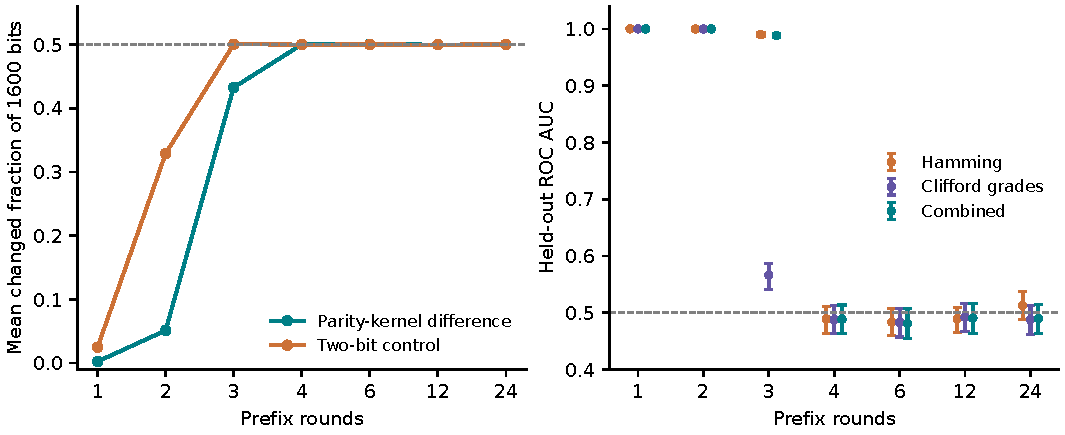
\includegraphics[width=\linewidth]{figures/diffusion_and_auc.pdf}
\caption{Left: mean state displacement. Right: held-out classification against uniform difference controls, with conditional bootstrap intervals. Checkpoints are displayed at equal spacing.}
\label{fig:diffusion}
\end{figure}

\begin{table}[htbp]
\centering\small
\AUCTable
\caption{Test AUC for fixed feature families. The true-difference class is positive, with score orientation chosen on training data. Scores below 0.5 are retained without a post-test sign flip.}
\end{table}

At three rounds, Hamming weight reaches AUC 0.9901; the Clifford grades alone reach 0.5661, and the combined model reaches 0.9885. Adding these particular Clifford features therefore does not improve the observed three-round score. At 24 rounds, combined AUC is 0.4897 with bootstrap interval $[0.4635,0.5144]$. For the 512 full-round digest-bit tests, the smallest raw $p$ is 0.00275, but none survives Holm correction at 0.05. These finite tests constrain the studied features and differences; they are not a security proof.

\subsection{Finite-feedback prediction}

\begin{table}[htbp]
\centering\small
\MarkovTable
\caption{Held-out average next-bin log loss over 24 transitions per trajectory. Lower is better. Intervals use 4,096 independent test trajectories.}
\end{table}

The full dyadic predictor improves over phase-only prediction by 0.018322 bits per transition, with a paired interval for the difference $[-0.020386,-0.016259]$. However, self-feedback increases loss relative to the same hierarchy without feedback by 0.002526 bits, with paired interval $[0.001150,0.003901]$. Thus the measured improvement is associated with conditioning and the dyadic hierarchy, while the selected feedback bit does not improve this prediction task. There are 540 observed meta contexts, and the maximum count is 4,096, below the finite cap. Predicting a coarse weight bin does not reconstruct a 256-bit digest or a satisfying preimage.

\subsection{Influence, structural SCCs, and projected cycles}

\begin{table}[htbp]
\centering\small
\CausalTable
\caption{Keccak-f[25] intervention and correlation summaries, averaged over 625 input/output pairs. Signed effects and Pearson correlations can cancel while flip influence remains large.}
\end{table}

\begin{figure}[htbp]
\centering
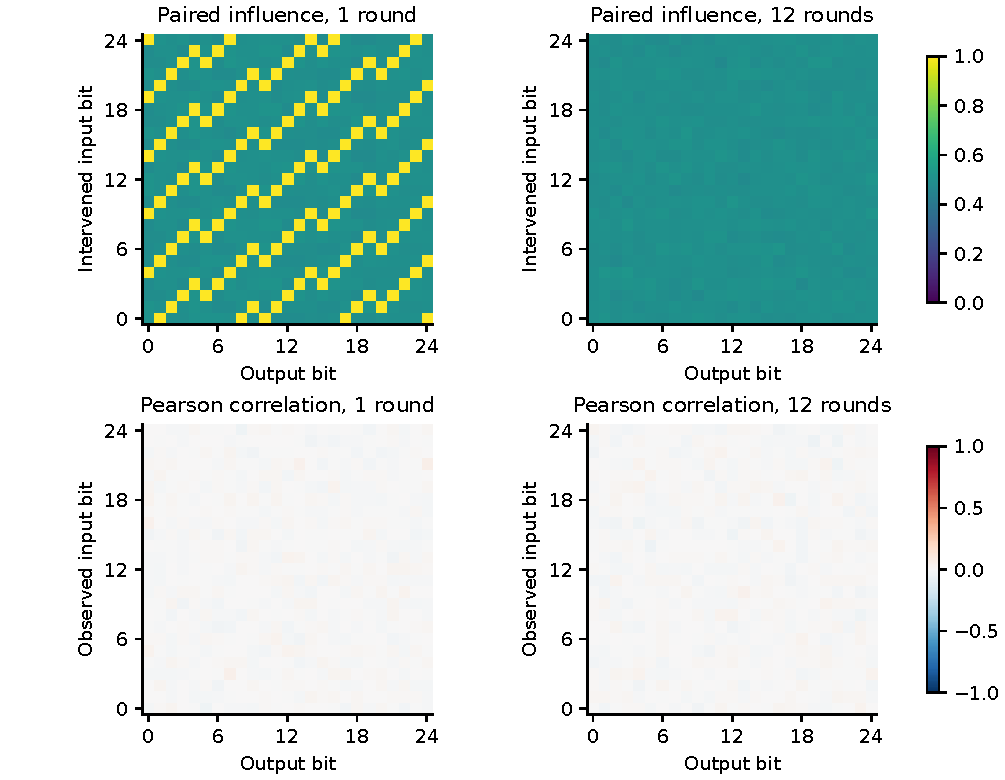
\includegraphics[width=0.90\linewidth]{figures/causal_influence.pdf}
\caption{Paired flip influence and observational Pearson correlation on the 25-bit permutation. Color scales are fixed across round counts; correlation is shown on its natural $[-1,1]$ scale.}
\end{figure}

The 1,600-coordinate structural graph contains 52,800 edges and one SCC of size 1,600. The 25-coordinate structural graph contains all 625 directed edges, also forming one SCC. In the sampled 25-bit influence graphs, thresholds 0.1 and 0.4 leave one component at every reported checkpoint. At threshold 0.6, the one-round graph has 125 edges and one SCC, whereas later sampled graphs have no edges. SCC structure therefore depends on the meaning and threshold of an edge; a large component is not by itself a cryptanalytic shortcut.

\begin{table}[htbp]
\centering\small
\CyclesTable
\caption{Exhaustive results for the 4,096-state projected/reinjected map $F_r$. These are not cycle counts of the full Keccak permutation.}
\end{table}

All projected maps and their cycle lengths are retained. As a descriptive control, 64 uniform random maps on the same number of vertices have a mean of 4.766 cycles and mean longest cycle 50.594. Intervals for these means are not prediction intervals for an individual map; we make no anomaly claim by comparing one observed cycle length to an interval for the null mean.

\subsection{Search and independent ablations}

\begin{table}[htbp]
\centering\small
\SearchTable
\caption{Primary twelve-bit target search. Every trial has a cap of 2,048 distinct-message queries. Exact paired success tests and their Holm adjustments are reported.}
\end{table}

\begin{figure}[htbp]
\centering
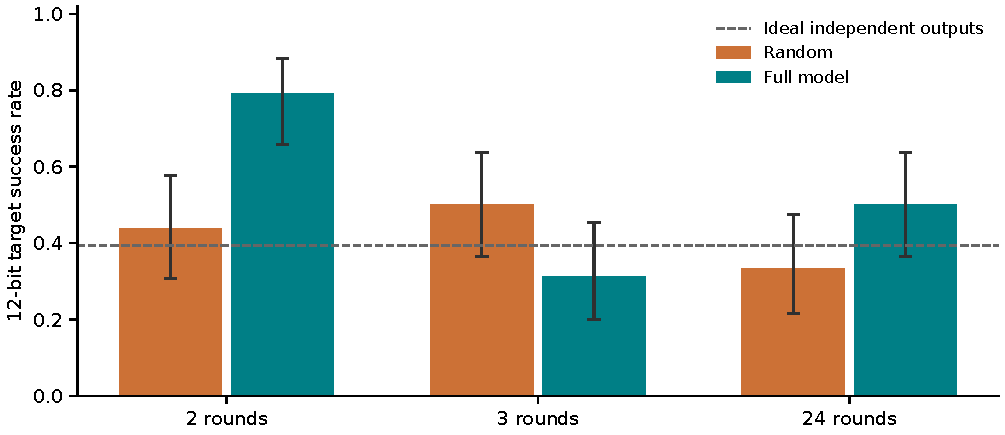
\includegraphics[width=0.94\linewidth]{figures/truncated_search.pdf}
\caption{Primary success rates with Wilson intervals. The dashed reference assumes independent ideal outputs. Success addresses a 12-bit target, not a 256-bit preimage.}
\end{figure}

The two-round primary result improves from 21/48 to 38/48 hits, with Holm-adjusted $p=0.00454$ over the three round counts. At three rounds the point estimate reverses, and at 24 rounds the exact paired result does not reject equal success. No conclusion is drawn from the small-sample $t$ interval on paired binary differences when it disagrees with the specified exact test.

\begin{table}[htbp]
\centering\small
\AblationTable
\caption{Independent-seed replication and ablations. Query columns are mean consumed queries, counting failures at the cap. No-SCC means the same fixed stagnation trigger without the SCC recurrence condition.}
\label{tab:ablation}
\end{table}

\begin{figure}[htbp]
\centering
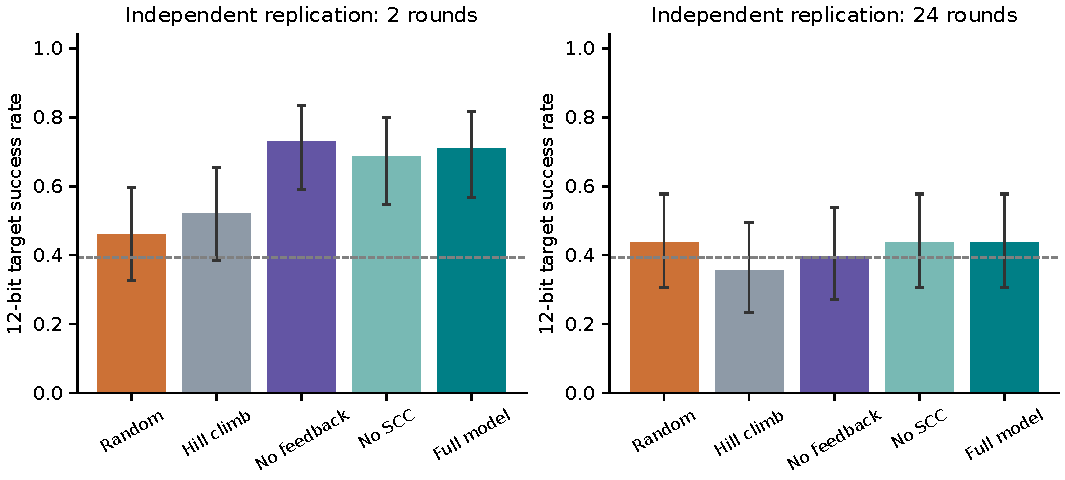
\includegraphics[width=\linewidth]{figures/search_ablations.pdf}
\caption{Follow-up search with new targets and seeds, 48 trials per method and round count. Bars and Wilson intervals show sampling uncertainty.}
\end{figure}

The independent two-round comparison gives 34/48 hits for the full model and 22/48 for random search, with nominal paired $p=0.02896$. Comparing all eight follow-up contrasts as one family would give no Holm rejection at 0.05; the replication supports the direction of the primary result without isolating a unique component. Uniform-action hill climbing obtains 25/48, removal of feedback obtains 35/48, and a simple stagnation restart obtains 33/48. The latter shares exactly the same endpoint and consumed-query count as the full model in 45/48 trials. Hence these measurements do not establish that self-reference or Tarjan SCCs are necessary for the observed two-round advantage. At 24 rounds, both full model and random search obtain 21/48, and the other ablations are compatible with sampling variation.

\FloatBarrier
\section{What the study establishes and what to test next}

The exact contribution is a concrete transport of SHA-3's Boolean round into an associative hypercomplex algebra, accompanied by a metric identity, a reproducible reduced collision family, and a local majority-closure obstruction to lossless 2-SAT replacement. The experimental contribution is a set of controlled measurements across three proposed analysis routes, including unfavorable ablations. It does not assume that changing number systems lowers the complexity of inversion, that a projected recurrence is a microscopic cycle, or that a more accurate diffusion predictor automatically yields a preimage.

The strongest measured search result is a small-output, two-round effect. Its operational target has only $2^{12}$ output values, and the query budget is already a substantial fraction of that space. Extrapolation to a 256-bit target, additional rounds, or asymptotic speedups would require a new argument and measurements at increasing target lengths. The measured Hamming-equivalent geometry alone cannot supply such an argument.

Useful follow-ups are to derive low-cost constraints from Clifford products beyond basis-dependent summary energies; test spatially richer finite contexts for approximate lumpability; preserve exact XOR and nonlinear constraints alongside SCC preprocessing; and replicate search at several truncation lengths with matched evaluation and wall-clock budgets. A controlled series should retain the simple hill-climbing and no-feedback baselines. The present repository gives the state representations, certificates, seeds, raw arrays, and verification tools needed to carry out those comparisons.

\section*{Reproducibility and attribution}

All code, result arrays, per-trial endpoint certificates, plotting scripts, LaTeX source, and this PDF are available at \url{https://github.com/PolloXDDD/SHA3-ANALISIS}. Numerical tables are generated from JSON results; figures are vector PDFs. The main run uses Python 3.12.14, NumPy 2.3.5, and SciPy 1.17.0. Source SHA-256 fingerprints appear in \texttt{results/manifest.json}; run times are descriptive and environment-specific. The author proposed the research directions. ChatGPT assisted with formalization, implementation, experiments, and manuscript drafting.

\bibliographystyle{plainnat}
\bibliography{references}

\clearpage
\appendix
\section{Reproduction commands and artifact map}

From the repository root, use a Python environment with the listed dependencies:
\begin{verbatim}
python -m pip install -r requirements.txt
python -m unittest discover -s tests -v
python -m sha3lab.experiments --out results
python -m sha3lab.ablations --out results
python scripts/verify_results.py
python scripts/build_report.py
python scripts/build_pdf.py
\end{verbatim}

The \texttt{--quick} flag on the main experiment is a smoke configuration; its outputs must be directed to a separate directory and must not replace the paper's dataset. The full study uses 8,192 pairs per fixed difference, 2,048 feature examples per class, 4,096 intervention contexts, exhaustive 4,096-state projected graphs, 288 primary search trials, and 480 follow-up trials.

\begin{center}\small
\begin{tabular}{p{.40\linewidth}p{.52\linewidth}}
\toprule
Artifact & Purpose\\
\midrule
\texttt{sha3lab/keccak.py} & Scalar and batched permutation; complete byte-aligned SHA-3.\\
\texttt{sha3lab/hypercomplex.py} & Clifford algebra, transported rounds, and grade features.\\
\texttt{sha3lab/metamarkov.py} & Dyadic predictor and controls.\\
\texttt{sha3lab/graphs.py} & SCC, exact 2-SAT, dependency graphs, local obstruction.\\
\texttt{sha3lab/attacks.py} & Collision construction and budgeted search policies.\\
\texttt{results/*.npz} & Raw weights, features, scores, matrices, and projected maps.\\
\texttt{results/*trials.json} & Every search endpoint, target, seed, and query count.\\
\texttt{tests/test\_lab.py} & Independent functional and mathematical checks.\\
\bottomrule
\end{tabular}
\end{center}

\end{document}
